\section{Gestion des terrains}

Cette section décrit comment gérer les terrains des propriétaires. En particulier, il est possible de consulter, modifier, valider, et supprimer ces terrains. \newline

Le gestionnaire des terrains est accessible via le menu de navigation sous le logo du site web, en cliquant sur l'onglet "Terrains".

\begin{figure}[H]
\centering
\includegraphics[scale=0.15]{user_images/staff/GererTerrains/001.jpg}
\caption{Gestionnaire des terrains}
\end{figure}

\subsection{Consulter un terrain}

Pour consulter un terrain parmi plusieurs terrains, il suffit de sélectionner un terrain dans la liste de tous les terrains à droite. Puisqu'il y a beaucoup de terrains, on peut filter les terrains en spécifiant des critères de recherche et/ou un champs de recherche.\newline

Les critères de recherche filtrent les terrains sur des critères bien spécifiques :

\begin{itemize}
\item la matière des terrains (terre battue, gazon, etc...)
\item la validation des terrains (validé ou non validé)
\item l'utilisation des terrains (utilisé ou non pour un tournoi)
\item la disponibilité des terrains (Samedi, Dimanche, ou les deux)
\item l'état du terrain (très bon, correct, etc...)
\item le type du terrain (ouvert, ou couvert)
\item le caractère vétéran du terrain (vétéran, non vétéran)
\item le nombre de résultats par page de la liste
\end{itemize}

Le champ de recherche permet de filter les terrains dont le texte correspond à une partie d'une information du terrain.\newline

Dans cet exemple, on souhaite avoir la liste de tous les terrains en terre battue, non validé, et ouvert, avec 10 résultats par page.

\begin{figure}[H]
\centering
\includegraphics[scale=0.15]{user_images/staff/GererTerrains/ConsulterTerrain/001.jpg}
\caption{Consulter un terrain, étape 1}
\end{figure}

Si on clique sur la première entrée, soit le terrain 69, on accède à la page de ce terrain.

\begin{figure}[H]
\centering
\includegraphics[scale=0.15]{user_images/staff/GererTerrains/ConsulterTerrain/002.jpg}
\caption{Consulter un terrain, étape 2}
\end{figure}

Sur cette page, on peut visualiser les informations du terrain sur la gauche. À droite, les commentaires du staff et l'état de validation du terrain y est indiqué. \newline

Dans la partie gauche, contenant les informations du terrain, il est possible de générer un document PDF du terrain, et éditer ce terrain. En bas de la page, un historique de toutes les modifications de ce terrain y est indiqué.

\begin{figure}[H]
\centering
\includegraphics[scale=0.15]{user_images/staff/GererTerrains/ConsulterTerrain/003.jpg}
\caption{Consulter un terrain, étape 3}
\end{figure}

\subsection{Valider un terrain}

Pour valider un terrain, il faut accéder à sa page, comme expliqué à la sous-section précédente (Consulter un terrain).

\begin{figure}[H]
\centering
\includegraphics[scale=0.15]{user_images/staff/GererTerrains/ValiderTerrain/001.jpg}
\caption{Valider un terrain, étape 1}
\end{figure}

Sur cette page, si le terrain n'est pas validé, alors la case "Terrain validé" n'est pas coché. Valider un terrain consiste simplement à cocher cette case, puis à cliquer sur le bouton "Valider".

\begin{figure}[H]
\centering
\includegraphics[scale=0.15]{user_images/staff/GererTerrains/ValiderTerrain/002.jpg}
\caption{Valider un terrain, étape 2}
\end{figure}

Un message au dessus des commentaires signale la bonne édition du terrain. En dessous de la page, l'historique du terrain contient une nouvelle entrée correspondant à la validation de ce terrain.

\begin{figure}[H]
\centering
\includegraphics[scale=0.15]{user_images/staff/GererTerrains/ValiderTerrain/003.jpg}
\caption{Valider un terrain, étape 3}
\end{figure}

\begin{figure}[H]
\centering

\includegraphics[scale=0.15]{user_images/staff/GererTerrains/ValiderTerrain/004.jpg}
\caption{Valider un terrain, étape 4}
\end{figure}

À la page principale de tous les terrains, on peut de nouveau remarquer que le terrain a bien été validé : un petit marqueur vert se trouve dans la colonne "Valide" de ce terrain, comme le montre la première entrée de l'image suivante.\newline

La validation d'un terrain permet de l'inclure dans la liste des terrains qui peuvent être utilisées pour gérer les tournois. En particulier, ce terrain peut être utilisé pour faire jouer une poule.

\begin{figure}[H]
\centering
\includegraphics[scale=0.15]{user_images/staff/GererTerrains/ValiderTerrain/005.jpg}
\caption{Valider un terrain, étape 5}
\end{figure}

\subsection{Editer un terrain}

Il est possible d'éditer un terrain en accédant tout d'abord à la page du terrain, comme expliqué dans la sous-section "Consulter un terrain".\newline

Sur cette page, cliquez sur le bouton "Editer Info" pour accéder à la page d'édition du terrain.

\begin{figure}[H]
\centering
\includegraphics[scale=0.15]{user_images/staff/GererTerrains/EditerInfosTerrain/001.jpg}
\caption{Editer un terrain, étape 1}
\end{figure}

Cette page est similaire à celle de l'édition d'un terrain pour le propriétaire : les champs du formulaire sont pré-remplis avec les données actuelles du terrain.\newline

\begin{figure}[H]
\centering
\includegraphics[scale=0.15]{user_images/staff/GererTerrains/EditerInfosTerrain/002.jpg}
\caption{Editer un terrain, étape 2}
\end{figure}

Sur l'image ci-dessous, nous avons modifié la matière du terrain en "Gazon", le type du terrain en "Ouvert", la disponibilité du terrain en "Samedi" et "Dimanche", et l'état du terrain en "Correct".\newline

Pour confirmer les modifications, cliquez sur le bouton "Editer" en bas de la page. 

\begin{figure}[H]
\centering
\includegraphics[scale=0.15]{user_images/staff/GererTerrains/EditerInfosTerrain/003.jpg}
\caption{Editer un terrain, étape 3}
\end{figure}

Sur la page principale du terrain, on remarque que le terrain a bien été édité. En bas de la page, l'historique des modifications contient une nouvelle entrée pour l'édition récente du terrain.

\begin{figure}[H]
\centering

\includegraphics[scale=0.15]{user_images/staff/GererTerrains/EditerInfosTerrain/004.jpg}
\caption{Editer un terrain, étape 4}
\end{figure}

\begin{figure}[H]
\centering
\includegraphics[scale=0.15]{user_images/staff/GererTerrains/EditerInfosTerrain/005.jpg}
\caption{Editer un terrain, étape 5}
\end{figure}

\subsection{Supprimer un terrain}

Cette sous-section explique comment supprimer un terrain. Pour commencer, l'utilisateur doit accéder à la page du terrain à supprimer, comme expliqué dans la sous-section "Consulter un terrain".\newline

Une fois sur la page du terrain à supprimer, cliquez sur le bouton "Editer Infos" pour accéder à la page d'édition du terrain.

\begin{figure}[H]
\centering
\includegraphics[scale=0.15]{user_images/staff/GererTerrains/SupprimerTerrain/001.jpg}
\caption{Supprimer un terrain, étape 1}
\end{figure}

Tout en bas de la page d'édition du terrain, cliquez sur le bouton de droite "Supprimer" pour supprimer ce terrain.

\begin{figure}[H]
\centering
\includegraphics[scale=0.15]{user_images/staff/GererTerrains/SupprimerTerrain/002.jpg}
\caption{Supprimer un terrain, étape 2}
\end{figure}

Comme cette action est irréversible, une boîte de dialogue demande à l'utilisateur de confirmer son action.

\begin{figure}[H]
\centering
\includegraphics[scale=0.15]{user_images/staff/GererTerrains/SupprimerTerrain/003.jpg}
\caption{Supprimer un terrain, étape 3}
\end{figure}

Après avoir validé l'action de suppression du terrain, le terrain est bien supprimé. Sur la page principale du gestionnaire des terrains, le terrain n'existe plus dans la liste des terrains.

\begin{figure}[H]
\centering

\includegraphics[scale=0.15]{user_images/staff/GererTerrains/SupprimerTerrain/004.jpg}
\caption{Supprimer un terrain, étape 4}
\end{figure}

Dans l'historique des modifications de tous les terrains, en bas de la page du gestionnaire des terrains, une nouvelle entrée indique la suppression de ce terrain.

\begin{figure}[H]
\centering
\includegraphics[scale=0.15]{user_images/staff/GererTerrains/SupprimerTerrain/005.jpg}
\caption{Supprimer un terrain, étape 5}
\end{figure}
